\section{Exploración de la dimensión del cromosoma}

\begin{table}[]
    \centering
    \begin{tabular}{|c|c|c|c|c|c|}
        \hline
        \textbf{Config.} & \textbf{DIM} & \textbf{\begin{tabular}[c]{@{}c@{}}Mediana \\ mejor valor \\ de fitness\end{tabular}} & \textbf{\begin{tabular}[c]{@{}c@{}}Mediana \\ \# ejecuciones \\ de f\end{tabular}} & \textbf{\begin{tabular}[c]{@{}c@{}}$\sigma$\\ mejor valor\\ de fitness\end{tabular}} & \textbf{\begin{tabular}[c]{@{}c@{}}$\sigma$\\ \# ejecuciones \\ de f\end{tabular}} \\ \hline
        10  [\ref{subsect:config_file_10}]               & 10           & -33.39                                                                                & 70902                                                                              & 4.23                                                                          & 15622.99                                                                    \\ \hline
        11  [\ref{subsect:config_file_11}]               & 15           & -24.28                                                                                & 138794.0                                                                           & 7.82                                                                          & 35438.36                                                                    \\ \hline
        12  [\ref{subsect:config_file_12}]               & 30           & 109.42                                                                                & 284149.0                                                                           & 14.18                                                                         & 65911.82                                                                    \\ \hline
        13  [\ref{subsect:config_file_13}]               & 50           & 367.07                                                                                & 512473.0                                                                           & 23.38                                                                         & 124996.18                                                                   \\ \hline
        14  [\ref{subsect:config_file_14}]               & 100          & 1327.54                                                                               & 1233227                                                                            & 50.60                                                                         & 217386.15                                                                   \\ \hline
    \end{tabular}
    \caption{Resultados exploración del tamaño del cromosoma, variando proporcionalmente el tamaño de población}
    \label{tab:exploracion_dim_cromosoma}
\end{table}

Para realizar esta exploración se ha seguido el mismo proceso que en las anteriores. El algoritmo se ha ejecutado 15 veces por cada fichero de configuración.
Se toma como base el tamaño de población 1000, que irá variando proporcionalmente a la dimensión del cromosoma. El resumen de estas ejecuciones está en la 
Tabla \ref{tab:exploracion_dim_cromosoma}. 

\begin{figure}[]
	\centering	
	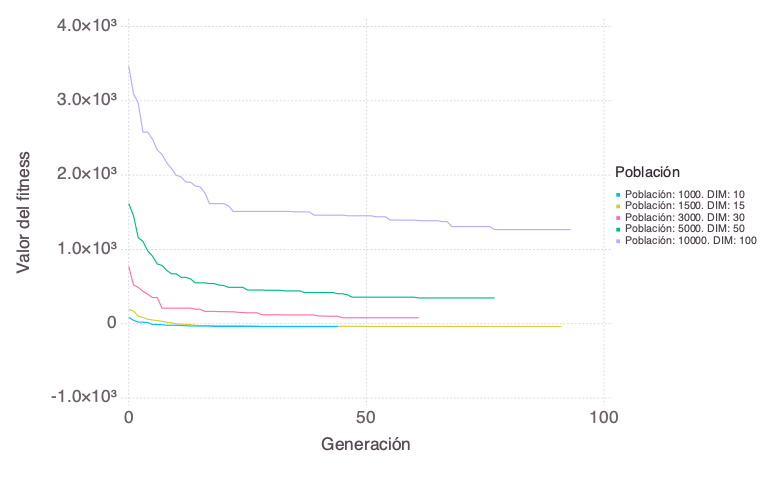
\includegraphics[scale=0.5]{../data/Plots/ps_cd_variation.png}
	\caption{ Variación del valor del fitness de cada fichero de configuración para la función Rastrigin a lo largo de las generaciones }
    \label{fig:exec_summary}
\end{figure}

\begin{figure}[]
	\centering	
	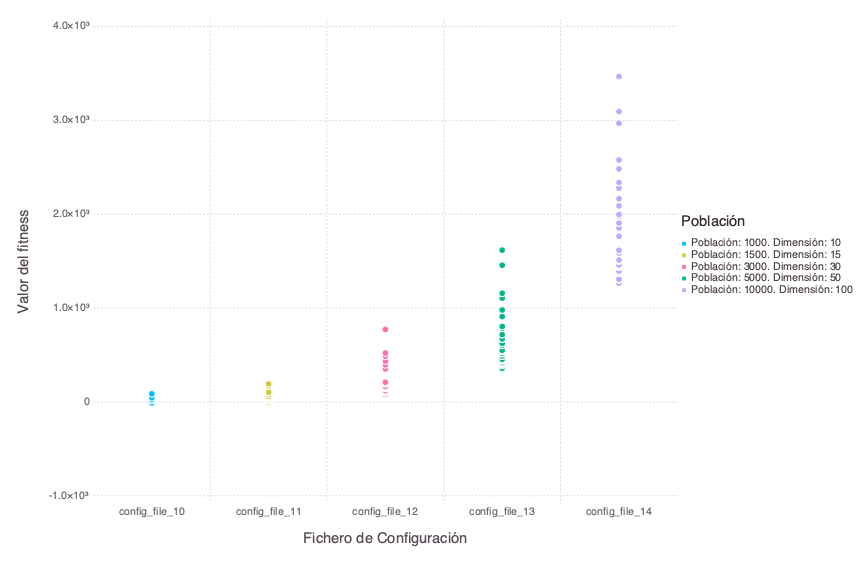
\includegraphics[scale=0.5]{../data/Plots/ps_cd_point.png}
	\caption{ Variación de los resultados, variando la dimensión del cromosoma }
    \label{fig:box_plots_crom_dim}
\end{figure}

Viendo la Figura \ref{fig:exec_summary}, todas las ejecuciones tienen un comportamiento parecido: gran descenso del valor del fitness al principio y estancamiento al final.
De esta exploración podemos concluir que aumentar el tamaño de la población proporcionalmente con la dimensión del cromosoma no consigue mejores resultados. Para la 
siguiente exploración se usará la configuración 13 [\ref{subsect:config_file_13}], por ver si cambiando la tasa de mutación se puede mejorar.